

\tikzset{every picture/.style={line width=0.75pt}} %set default line width to 0.75pt        

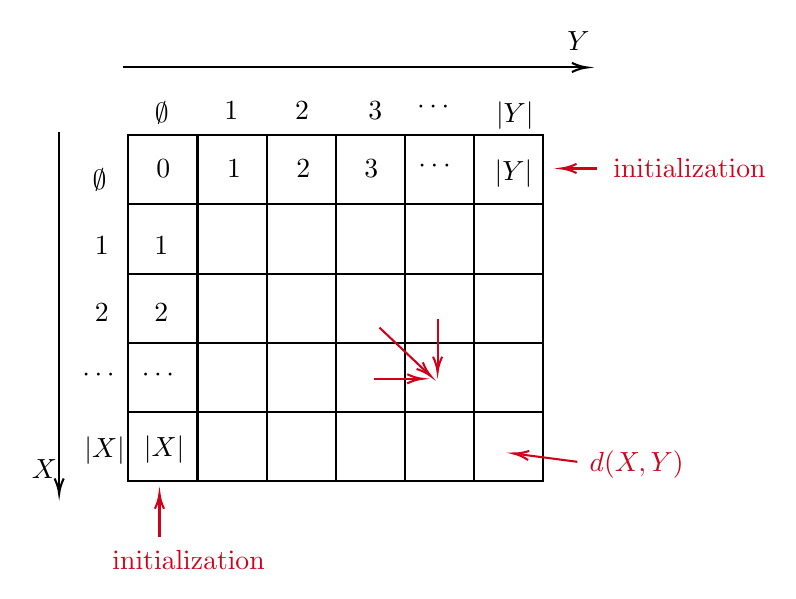
\begin{tikzpicture}[x=0.5pt,y=0.5pt,yscale=-1,xscale=1]
%uncomment if require: \path (0,424); %set diagram left start at 0, and has height of 424

%Shape: Grid [id:dp9095284515127875] 
\draw  [draw opacity=0] (87,90) -- (387,90) -- (387,340) -- (87,340) -- cycle ; \draw   (137,90) -- (137,340)(187,90) -- (187,340)(237,90) -- (237,340)(287,90) -- (287,340)(337,90) -- (337,340) ; \draw   (87,140) -- (387,140)(87,190) -- (387,190)(87,240) -- (387,240)(87,290) -- (387,290) ; \draw   (87,90) -- (387,90) -- (387,340) -- (87,340) -- cycle ;
%Straight Lines [id:da5347307434268296] 
\draw    (37,88) -- (37,347) ;
\draw [shift={(37,349)}, rotate = 270] [color={rgb, 255:red, 0; green, 0; blue, 0 }  ][line width=0.75]    (10.93,-3.29) .. controls (6.95,-1.4) and (3.31,-0.3) .. (0,0) .. controls (3.31,0.3) and (6.95,1.4) .. (10.93,3.29)   ;
%Straight Lines [id:da4989887299865372] 
\draw    (83,41) -- (416.5,41) ;
\draw [shift={(418.5,41)}, rotate = 180] [color={rgb, 255:red, 0; green, 0; blue, 0 }  ][line width=0.75]    (10.93,-3.29) .. controls (6.95,-1.4) and (3.31,-0.3) .. (0,0) .. controls (3.31,0.3) and (6.95,1.4) .. (10.93,3.29)   ;
%Straight Lines [id:da0785458532791945] 
\draw [color={rgb, 255:red, 208; green, 2; blue, 27 }  ,draw opacity=1 ]   (425.5,114) -- (402,114) ;
\draw [shift={(400,114)}, rotate = 360] [color={rgb, 255:red, 208; green, 2; blue, 27 }  ,draw opacity=1 ][line width=0.75]    (10.93,-3.29) .. controls (6.95,-1.4) and (3.31,-0.3) .. (0,0) .. controls (3.31,0.3) and (6.95,1.4) .. (10.93,3.29)   ;
%Straight Lines [id:da6572289654883201] 
\draw [color={rgb, 255:red, 208; green, 2; blue, 27 }  ,draw opacity=1 ]   (109.5,380) -- (109.5,351) ;
\draw [shift={(109.5,349)}, rotate = 450] [color={rgb, 255:red, 208; green, 2; blue, 27 }  ,draw opacity=1 ][line width=0.75]    (10.93,-3.29) .. controls (6.95,-1.4) and (3.31,-0.3) .. (0,0) .. controls (3.31,0.3) and (6.95,1.4) .. (10.93,3.29)   ;
%Straight Lines [id:da5210331041787328] 
\draw [color={rgb, 255:red, 208; green, 2; blue, 27 }  ,draw opacity=1 ]   (411.5,326) -- (367.48,320.26) ;
\draw [shift={(365.5,320)}, rotate = 367.43] [color={rgb, 255:red, 208; green, 2; blue, 27 }  ,draw opacity=1 ][line width=0.75]    (10.93,-3.29) .. controls (6.95,-1.4) and (3.31,-0.3) .. (0,0) .. controls (3.31,0.3) and (6.95,1.4) .. (10.93,3.29)   ;
%Straight Lines [id:da7955919237642329] 
\draw [color={rgb, 255:red, 208; green, 2; blue, 27 }  ,draw opacity=1 ]   (310.5,223) -- (310.5,259) ;
\draw [shift={(310.5,261)}, rotate = 270] [color={rgb, 255:red, 208; green, 2; blue, 27 }  ,draw opacity=1 ][line width=0.75]    (10.93,-3.29) .. controls (6.95,-1.4) and (3.31,-0.3) .. (0,0) .. controls (3.31,0.3) and (6.95,1.4) .. (10.93,3.29)   ;
%Straight Lines [id:da8723913218756593] 
\draw [color={rgb, 255:red, 208; green, 2; blue, 27 }  ,draw opacity=1 ]   (264.5,266) -- (297.5,266) ;
\draw [shift={(299.5,266)}, rotate = 180] [color={rgb, 255:red, 208; green, 2; blue, 27 }  ,draw opacity=1 ][line width=0.75]    (10.93,-3.29) .. controls (6.95,-1.4) and (3.31,-0.3) .. (0,0) .. controls (3.31,0.3) and (6.95,1.4) .. (10.93,3.29)   ;
%Straight Lines [id:da007837806914727685] 
\draw [color={rgb, 255:red, 208; green, 2; blue, 27 }  ,draw opacity=1 ]   (268.5,229) -- (304.05,262.63) ;
\draw [shift={(305.5,264)}, rotate = 223.41] [color={rgb, 255:red, 208; green, 2; blue, 27 }  ,draw opacity=1 ][line width=0.75]    (10.93,-3.29) .. controls (6.95,-1.4) and (3.31,-0.3) .. (0,0) .. controls (3.31,0.3) and (6.95,1.4) .. (10.93,3.29)   ;

% Text Node
\draw (68,103) node [anchor=north west][inner sep=0.75pt]   [align=left] {$ $};
% Text Node
\draw (60.5,161.38) node [anchor=north west][inner sep=0.75pt]   [align=left] {$\displaystyle 1$};
% Text Node
\draw (51.5,257.14) node [anchor=north west][inner sep=0.75pt]   [align=left] {$\displaystyle \cdots $};
% Text Node
\draw (15,322) node [anchor=north west][inner sep=0.75pt]   [align=left] {$\displaystyle X$};
% Text Node
\draw (402,13) node [anchor=north west][inner sep=0.75pt]   [align=left] {$\displaystyle Y$};
% Text Node
\draw (104,63.44) node [anchor=north west][inner sep=0.75pt]   [align=left] {$\displaystyle \emptyset $};
% Text Node
\draw (293.4,63.44) node [anchor=north west][inner sep=0.75pt]   [align=left] {$\displaystyle \cdots $};
% Text Node
\draw (59,112) node [anchor=north west][inner sep=0.75pt]   [align=left] {$\displaystyle \emptyset $};
% Text Node
\draw (60.5,209.76) node [anchor=north west][inner sep=0.75pt]   [align=left] {$\displaystyle 2$};
% Text Node
\draw (53,305.5) node [anchor=north west][inner sep=0.75pt]   [align=left] {$\displaystyle | X|$};
% Text Node
\draw (154.1,63.44) node [anchor=north west][inner sep=0.75pt]   [align=left] {$\displaystyle 1$};
% Text Node
\draw (205.2,63.44) node [anchor=north west][inner sep=0.75pt]   [align=left] {$\displaystyle 2$};
% Text Node
\draw (350.5,63.44) node [anchor=north west][inner sep=0.75pt]   [align=left] {$\displaystyle | Y|$};
% Text Node
\draw (258.3,63.44) node [anchor=north west][inner sep=0.75pt]   [align=left] {$\displaystyle 3$};
% Text Node
\draw (105.1,105.44) node [anchor=north west][inner sep=0.75pt]   [align=left] {$\displaystyle 0$};
% Text Node
\draw (156.1,105.44) node [anchor=north west][inner sep=0.75pt]   [align=left] {$\displaystyle 1$};
% Text Node
\draw (206.2,105.44) node [anchor=north west][inner sep=0.75pt]   [align=left] {$\displaystyle 2$};
% Text Node
\draw (255.3,105.44) node [anchor=north west][inner sep=0.75pt]   [align=left] {$\displaystyle 3$};
% Text Node
\draw (294.4,105.44) node [anchor=north west][inner sep=0.75pt]   [align=left] {$\displaystyle \cdots $};
% Text Node
\draw (349.5,105.44) node [anchor=north west][inner sep=0.75pt]   [align=left] {$\displaystyle | Y|$};
% Text Node
\draw (103.5,160.88) node [anchor=north west][inner sep=0.75pt]   [align=left] {$\displaystyle 1$};
% Text Node
\draw (94.5,256.64) node [anchor=north west][inner sep=0.75pt]   [align=left] {$\displaystyle \cdots $};
% Text Node
\draw (103.5,209.26) node [anchor=north west][inner sep=0.75pt]   [align=left] {$\displaystyle 2$};
% Text Node
\draw (96,305) node [anchor=north west][inner sep=0.75pt]   [align=left] {$\displaystyle | X|$};
% Text Node
\draw (435.3,104.44) node [anchor=north west][inner sep=0.75pt]   [align=left] {\textcolor[rgb]{0.82,0.01,0.11}{initialization}};
% Text Node
\draw (73.3,387.44) node [anchor=north west][inner sep=0.75pt]   [align=left] {\textcolor[rgb]{0.82,0.01,0.11}{initialization}};
% Text Node
\draw (418.2,315.44) node [anchor=north west][inner sep=0.75pt]   [align=left] {$\displaystyle \textcolor[rgb]{0.82,0.01,0.11}{d( X,Y)}$};


\end{tikzpicture}

